\chapter{設計と実装}
\label{chap:implementation}
本章ではRive日本語入力全体の設計と、
構成する各システムについての詳細な実装の解説を行う。

\newpage
\section{Rive日本語入力システム}
Rive日本語入力システムは以下のものによって構成されている。
\begin{itemize}
  \item Rive Client
  \item Rive Server
  \item Rive Analytics
  \item Rive Batchprocessing
  \item Rive Webservice
  \item DataBase
\end{itemize}
これらのシステムがお互いに作用することで
Rive日本語入力システムを実現している。
(システム全体構成図:\ref{fig:systemstructure})
\begin{figure}[htbp]
  \begin{center}
    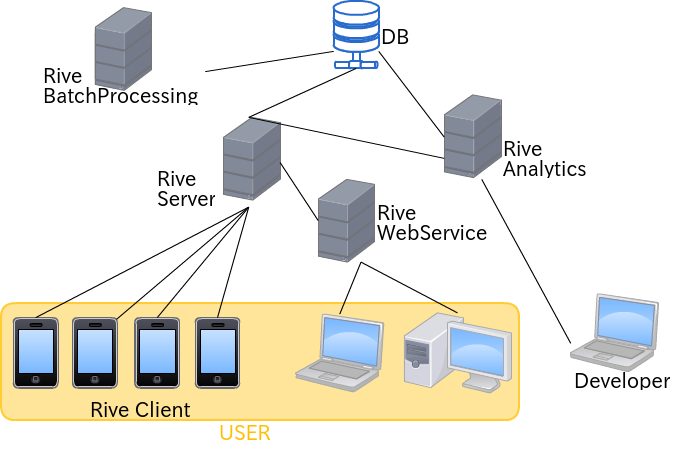
\includegraphics[width=120mm,bb=0 0 540 448]{images/systemstructure.png}
  \end{center}
  \caption{システム全体構成図}
  \label{fig:systemstructure}
\end{figure}

\section{Rive Client}
\label{sec:riveclient}
本システムはAndroidOS上で動くアプリケーション
として実装した。
ユーザは本アプリケーションをインストールし、
使用するIMEに選択することで
Rive日本語入力を利用することが可能である。
(Rive Clientユーザ画面:\ref{fig:riveclient})
\begin{figure}[htbp]
  \begin{center}
    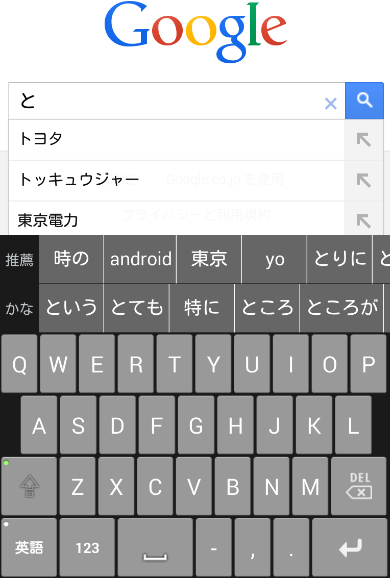
\includegraphics[width=140mm,bb=0 0 390 578]{images/riveclient.png}
  \end{center}
  \caption{Rive Clientユーザー画面}
  \label{fig:riveclient}
\end{figure}

\subsection{システムフロー}
このシステムが立ち上がるとまず始めにonCreate()メソッド
が呼ばれ、システムのイニシャライズを行う。
その後onStartInput()メソッドが呼ばれコンテキストを取得する。
ここで取得するコンテキストは静的コンテキストと
動的コンテキストの両方である。
コンテキストを取得し次第、この候補単語はサーバーと通信した上で
推薦候補単語を取得する。
これをユーザーが一つの操作を行うたびに繰り返す。
ここで言う一つの動作とは、
キーボード上の一つの文字を押すことであるonKeyDown()メソッドや、
候補の単語をタッチするpickCandidateWord()メソッド、
あるいは文字をデリートするdeleteWord()メソッドも含まれる。
二回目移行のコンテキスト取得においては動的コンテキストのみの取得となる。
最終的にユーザーが入力を終了した場合にはonFinishInput()が呼ばれ、
今回のユーザが行った動作とコンテキストを紐付けサーバーに送信する。
通信が終わり次第onDestory()が呼ばれ本システムは終了する。
(システムフローイメージ図:\ref{fig:clientflow})
\begin{figure}[htbp]
  \begin{center}
    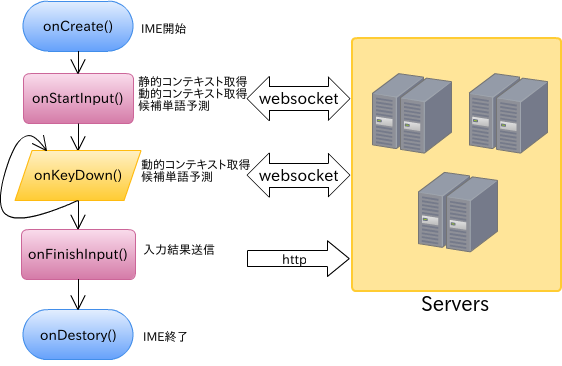
\includegraphics[width=140mm,bb=0 0 562 366]{images/clientflow}
  \end{center}
  \caption{Rive Clientフローイメージ}
  \label{fig:clientflow}
\end{figure}

\subsection{コンテキスト取得}
取得するコンテキストについては\ref{sec:getcontext}項を参照。
物理的なセンシングからは推測が困難であるが、
有用であると考えられるコンテキストは
設定画面においてユーザーが入力を行う。
その他デバイスで取得可能なものを全て取得し、推薦システムに使う。

\section{Rive Server}
\label{sec:riveserver}
Rive日本語入力における適切な候補単語を推測するサーバー郡の総称である。
Rive Clientからコンテキストデータを受け取り、
集合知を用いて解析を行う。
解析し適した候補単語を推測し、それら候補単語をRive Clientに送信する。
またRive Analyticsに入力データを送信するという役割も担っている。

\subsection{システム構成}
サーバーの中身は大きくRoutting Server,beforeRules,afterRules,Jubatusの
4つから成り立っている。
Routing Serverは非同期処理に適した
Node.js\footnote{http://nodejs.jp/}によって実装した。
それぞれ候補単語の計算手法が異なるため(図:\ref{fig:riveserver})
ような分割になっている。
\begin{figure}[htbp]
  \begin{center}
    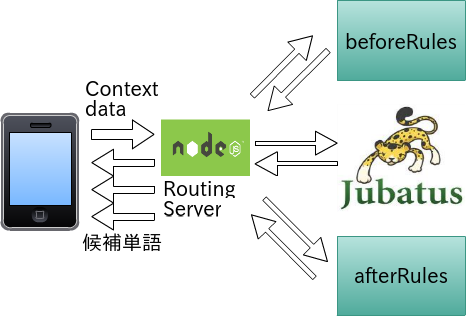
\includegraphics[width=14cm,bb=0 0 466 316]{images/riveserver.png}
  \end{center}
  \caption{Rive Server概要図}
  \label{fig:riveserver}
\end{figure}
始めにクライアントがコンテキストデータをRouting Serverへ送信する。
その後Routing ServerがbeforeRulesへコンテキストデータを送る。
beforeRulesは送られてきたデータを元に推薦候補単語をRouting Serverに送る。
Routing Serverは受け取ったデータをクライアントに返すと共に、
Jubatusへコンテキストデータを再送する。
Jubatusはそのデータを元に推薦候補単語を推測しRouting Serverへ送る。
Routing Serverは受け取ったデータを更にクライアントへ送る。
そしてそれと共にコンテキストデータをafterRulesに再送する。
そのデータを元に推薦候補単語をRouting Serverへ送る。
そしてそれをクライントに返すことで完了する。
一回のタッチごとにこれら全てのプロセスを行う。
クライアントは非同期に受け取った推薦候補単語をスコア順にソートして表示する。
またこれらの一度の過程ごとにユニークなIDをつけてあり、
途中で新しいプロセスが始まった場合前のプロセスは破棄されることで
常に最新の推薦候補単語を受け取ることができる。

\subsection{Routing Server}
Routing Serverは二通りの役割を担っている。
一つはデバイスから受け取ったコンテキストデータを
beforeRules,Jubatus,afterRulesの3つの計算エンジン
のどれに振り分けるかを判断し、それぞれに送信する役割である。
もう一つはデータを受け取り次第、デバイスに返信する役割である。

\subsection{beforeRules}
\label{sec:beforerules}
このエンジンはコンテキストデータが送られてきた際に、
一定のルールに基づいて推薦候補を計算するものをまとめている。
このルールは開発者がよく使う単語を推測し実装した。
例えば、Twitter\footnote{http://twitter.com/}
クライアントに入力を行っている(行おうとしている)
場合に「なう」「@」の候補単語を返すようになっている。

\subsection{Jubatus}
このエンジンについては\ref{sec:jubatus}項参照。

\subsection{afterRules}
\label{sec:afterrules}
このエンジンはbeforeRulesより重要度が低く、
また計算に時間がかかるものを推測して実装した。
例えば、最寄り駅をクエリとしてその駅を通っている電車の線を
その場でWEBから検索し推薦単語として返すという処理などである。

\section{Rive Analytics}
このシステムはRive Clientでのプロセスの終わりに
送られてくる入力データを受け取り、解析するシステムである。
開発者はこのシステムを開発時に使用することによって、
新しい機能の有用性などを確かめることができる。
バージョン管理システムであるgit\footnote{http://git-scm.com}
のcommit\footnote{http://git-scm.com/docs/git-commit}
とデータを紐付けて入力データを管理する。
ユーザーは直接本システムとの関わりは持たない。

\subsection{指標値に用いる単語の説明}
\begin{description}
  \item[click] デバイスにおける全てのタッチ
  \item[touch] 候補単語のタッチ
  \item[before] beforeRules(\ref{sec:beforerules}項)からのタッチ
  \item[after] afterRules(\ref{sec:afterrules}項)からのタッチ
  \item[jubatus] Jubatus(\ref{sec:jubatus}項)からのタッチ
  \item[recommend] beforeRulesとafterRulesとJubatusの総和からのタッチ
  \item[score] Jubatusにおいて算出したスコア
\end{description}
\subsection{指標値}
\begin{itemize}
  \item CPI - Click Per Input\mbox{}\\
    この指標値は一度の入力に対して
    平均でどれくらいクリックしたかを示している値である。
    値を低く保つことで入力の省入力化を達成できる。
  \item msPI - milliseconds Per Input\mbox{}\\
    この指標値は一度の入力に対して
    平均で何ミリ秒かかったかを示している値である。
    値を低く保つことで入力の省入力化を達成できる。
  \item TPI - Touch Candidate Per Input\mbox{}\\
    この指標値は一度の入力に対して
    平均で何度候補単語をタッチしたかを示している値である。
    推薦エンジンの有用性を示す値となる。
  \item TPC - Touch Candidate per Click\mbox{}\\
    この指標値はクリック回数のうち
    候補単語がタッチされた割合を示す値である。
    割合を把握することで、
    キーボードと候補のどちらを改善すべきかを示す値である。
  \item RPC - Recommend Per Touch\mbox{}\\
    この指標値は候補単語をタッチされた回数のうち
    どれだけの割合で推薦候補をタッチされたかを示す値である。
    この値を高めることで推薦エンジンの有用性を示す。
  \item Score - Score average by Jubatus\mbox{}\\
    この指標値はJubatusによる推薦単語がタッチされた時に、
    いくつのスコアのものがタッチされたかを示す値である。
    beforeRulesやafterRulesの閾値の参考にする値である。
  \item BPR - Before rules Per Recommend\mbox{}\\
    この指標値は推薦単語がタッチされたうちの
    beforeRulesのタッチされた割合を示す値である。
    beforeRulesの有用性を示す値となる。
  \item APR - After rules Per Recommend\mbox{}\\
    この指標値は推薦単語がタッチされたうちの
    afterRulesのタッチされた割合を示す値である。
    afterRulesの有用性を示す値となる。
  \item JPR - Jubatus Per Recommend\mbox{}\\
    この指標値は推薦単語がタッチされたうちの
    Jubatusからきた推薦単語のタッチされた割合を示す値である。
    Jubatusからくる推薦単語の有用性を示している。
  \item JPT - Jubatus Per Touch\mbox{}\\
    この指標値は候補単語をタッチした回数のなかで
    Jubatusからくる推薦単語の割合を示す値である。
    jubatusからくる推薦単語の有用性を示している。
\end{itemize}
これらをgitのcommitとひもづけることによってバージョンごとに
データを管理している。(図:\ref{fig:riveanalytics})
\begin{figure}[htbp]
  \begin{center}
    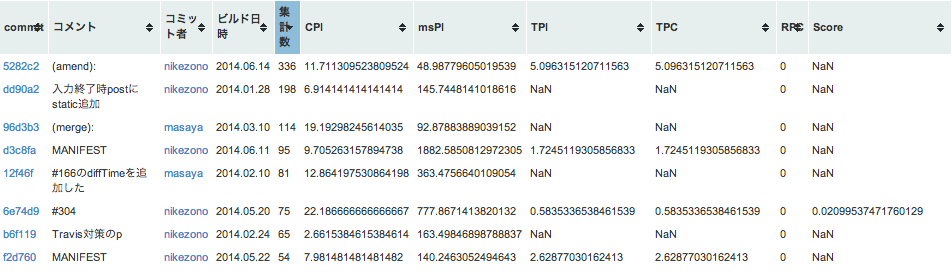
\includegraphics[width=170mm,bb=0 0 952 274]{images/riveanalytics.png}
    \caption{Rive Analytics画面}
    \label{fig:riveanalytics}
  \end{center}
\end{figure}
必要な指標値と開発におけるバージョンを見比べながら
有効であると思われる機能についての開発の参考にする。

\section{Rive Batchprocessing}
このシステムは定期的に処理を行うものを管理し実行している。
インターネット上のデータをクロールし、
DBを定期的にアップデートするプログラムなどが構成している。

\section{Rive Webservice}
このシステムはインターネット上で利用可能なWebページとして実装した。
Rive Serverの推薦を試用することができ、
またRive日本語入力の使い方などを説明している。
\footnote{http://rive.in}
Rive Serverと通信を行い、
Rive Webservice上で仮想のコンテキストを設定することで、
どのような推薦候補単語を受け取ることができるか
シミュレーションすることができる。
(体験画面イメージ:\ref{fig:rivewebservice})
\begin{figure}[htbp]
  \begin{center}
    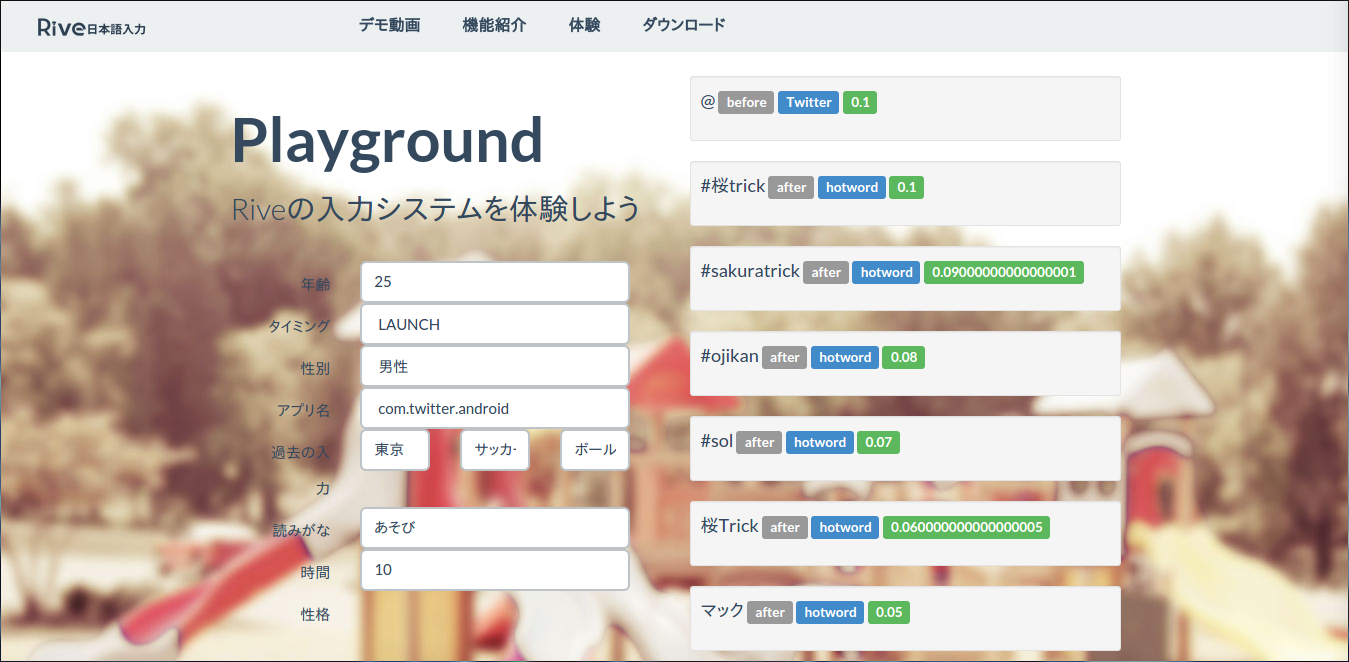
\includegraphics[width=160mm,bb=0 0 1349 662]{images/rivewebservice.png}
    \caption{Rive Webserviceの体験画面}
    \label{fig:rivewebservice}
  \end{center}
\end{figure}

\section{データベース}
取得するコンテキスト共に、
スキーマが頻繁に変わるため
スキーマの変更に対応しやすいNoSQLデータベースである、
MongoDB\footnote{http://www.mongodb.org/}を採用した。

\section{システム間通信}
Rive ClientとRive Server間の通信は
Websocket\footnote{http://dev.w3.org/html5/websocket/}、
その他のシステム間はhttpによって実現した。
Websocketを採用した理由はサーバー側からのプッシュ機構
を導入するためと、
httpより速度が早いためという理由である\cite{websocket}。
